\chapter{Implementacja}

Rozdział ten zawiera wszystkie informacje dotyczące aplikacji noszącej nazwę Graphy, która została napisana w ramach tej pracy. 

Przedstawię w nim użyte narzędzia i biblioteki oraz architekturę systemu. Opiszę również działanie aplikacji: które funkcjonalności udało mi się zaimplementować, a które wymagają dalszej pracy. 

Znajdzie się tutaj również sekcja o testach aplikacji (jednostkowych, \textit{end-to-end} oraz manualnych). Następnie pojawią się bardziej techniczne informacje dla programistów, opisujące w jaki sposób zrealizować typowe zadanie takie jak: dodanie nowego algorytmu, parsera czy skrótu klawiszowego. Na samym końcu przedstawię pomysły, w jaki sposób można dalej rozwijać aplikację.

\section{Podstawowe informacje}

Aplikacja została napisana w języku TypeScript -- wolnym i otwartym języku programowania stworzonym przez firmę Microsoft, który jest nadzbiorem języka JavaScript i który transpiluje się do JavaScriptu. Umożliwia on statyczną kontrolę typów oraz programowanie zorientowane obiektowo oparte na klasach.

Projekt korzysta z systemu kontroli wersji Git i jego repozytorium kodu znajduje się w serwisie GitHub. Wersja demonstracyjna aplikacji jest udostępniona na serwerach GitHub Pages. Adresy repozytorium i wersji demonstracyjnej znajdują się w poniższej tabeli.

\bigskip
\noindent\begin{tabularx}{\textwidth}{r|X|}
\cline{2-2}
  Repozytorium kodu & \hyperref[https://github.com/lukaszkostrzewa/graphy]{https://github.com/lukaszkostrzewa/graphy} \\ 
\cline{2-2} 
 Wersja demonstracyjna & \hyperref[https://lukaszkostrzewa.github.io]{https://lukaszkostrzewa.github.io} \\ 
\cline{2-2}
\end{tabularx} 
\bigskip

Jest to aplikacja \textit{front-endowa}. Oznacza to, że w chwili obecnej nie komunikuje się ona z serwerem ani zewnętrznymi serwisami (np. w celu zapisania czy zaimportowania grafu). Wszystkie operacje są wykonywane po stronie klienta, tzn. po stronie przeglądarki internetowej. Przy dalszym rozwoju aplikacji konieczne może okazać się napisanie drugiej, odseparowanej aplikacji pełniącej rolę \textit{back-endu}, która będzie wystawiać serwisy umożliwiające komunikację z bazą danych czy z innymi użytkownikami (np. udostępnianie grafu w czasie rzeczywistym).

Aplikacja została udostępniona na licencji MIT. Poniższa tabela przedstawia podstawowe statystyki dotyczące projektu.

\bigskip
\begin{table}[H]
\begin{threeparttable}
\centering
\noindent\begin{tabularx}{\textwidth}{r|X|}
\cline{2-2}
  Liczba linii kodu\tnote{1} & 8137 \\ 
\cline{2-2}
  Liczba plików\tnote{1} & 151 \\ 
\cline{2-2}
 Rozmiar kodu\tnote{1} & 270 KB \\ 
\cline{2-2}
 Ilość zatwierdzonych zmian w Git\tnote{2} & 112 \\ 
\cline{2-2}
 Pokrycie testami jednostkowymi\tnote{3} & 74.57\% \\ 
\cline{2-2}
\end{tabularx} 
\begin{tablenotes}
{\footnotesize\medskip
\item[1] nie licząc kodu zewnętrznych bibliotek
\item[2] ang. \textit{commits}
\item[3] procent pokrytych linii kodu
}
\end{tablenotes}
\end{threeparttable}
\end{table}
\bigskip


\section{Biblioteki i narzędzia}

W aplikacji jako biblioteka do wizualizacji grafów została użyta biblioteka Cytoscape.js. Posiada ona bardzo przyjazne API, obszerną dokumentację zawierającą gotowe przykłady oraz szereg dodatków, które rozszerzają podstawowe funkcjonalności. Ogromnym plusem biblioteki jest to, że jest aktywnie rozwijana, posiada dużą społeczność i wsparcie -- jej główny kontrybutor Max Franz odpowiada na każdą wiadomość w serwisach Stack Overflow oraz GitHub. Kolejnymi zaletami są architektura biblioteki oraz wsparcie dla urządzeń mobilnych.

Aplikacja została napisana przy użyciu biblioteki Angular, która została stworzona i jest rozwijana przez firmę Google. Projekt został wygenerowany przez narzędzie Angular CLI (ang. \textit{command line interface}). Narzędzie to umożliwia szybki start z biblioteką Angular -- pozwala na wygenerowanie już skonfigurowanego projektu, dostarcza komendy do generowania nowych komponentów, serwisów czy dyrektyw, do uruchamiania testów jednostkowych oraz testów \textit{end-to-end} oraz zawiera w sobie serwer programistyczny, który oferuje możliwość automatycznego przeładowywania aplikacji po wykryciu zmiany w kodzie źródłowym. 

Angular w wersji 2 (i nowszej) korzysta z języka TypeScript. Dzięki niemu i dzięki statycznej kontroli typów, którą język ten oferuje, możemy wcześniej uniknąć błędów programistycznych, już w momencie pisania kodu, a nie w momencie uruchomienia. Ponadto język ten oferuje szereg elementów z nadchodzących edycji ECMAScript\footnote{ECMAScript -- specyfikacja skryptowego języka stworzona i rozwijana przez organizację Ecma International, którą implementuje m.in. JavaScript.} takich jak moduły, klasy, interfejsy oraz wiele innych. Pozwala to na pisanie kodu modułowego, który jest łatwiejszy w utrzymaniu, testowaniu i rozwijaniu.

Ponadto w projekcie wykorzystywane są narzędzia do testowania domyślnie dostarczane w projekcie wygenerowanym przez Angular CLI: Karma i Protractor. Ich dokładniejszy opis znajduje się w sekcji \ref{sec:tests} Testy.

\section{Architektura}

Projekt składa się z 19 \emph{komponentów} (\texttt{@Component}). Każdy komponent mieści się w osobnym katalogu, w którym (zgodnie z konwencją zalecaną w Angularze) znajdują się: 
\begin{itemize}
\setlength\itemsep{0em}
\item plik \texttt{*.html} odpowiadający za widok, 
\item plik \texttt{*.scss} będący arkuszem styli Sass\footnote{Sass (ang. \textit{Syntactically Awesome Style Sheets}) -- jest to rozszerzenie języka CSS wzbogacającym go o takie funkcjonalności jak dziedziczenie, zagnieżdżanie styli, stosowanie zmiennych czy importowanie styli z innych plików.}, 
\item plik \texttt{*.ts} zawierający kod z klasą komponentu,
\item oraz plik \texttt{*.spec.ts} z testami jednostkowymi komponentu. 
\end{itemize}

Głównym komponentem jest \texttt{GraphComponent}, w którym jest inicjalizowany obiekt Cytoscape. Korzysta on z \emph{serwisów} (\texttt{@Injectable}), aby zaimportować graf, wyeksportować graf lub uruchomić na nim algorytm.

Oprócz tego w projekcie znajduje się szereg \emph{dyrektyw} (\texttt{@Directive}), które pełnią funkcję rozszerzeń (np. menu kontekstowe, dodatek odpowiadający za wyginanie krawędzi czy dodatek odpowiadający za rejestrację i obsługę skrótów klawiszowych).

Zarys architektury wraz z zaznaczonymi ważniejszymi komponentami, serwisami i dyrektywami został przedstawiony na rysunku \ref{fig:architecture}.

\begin{figure}[H]
\centerline{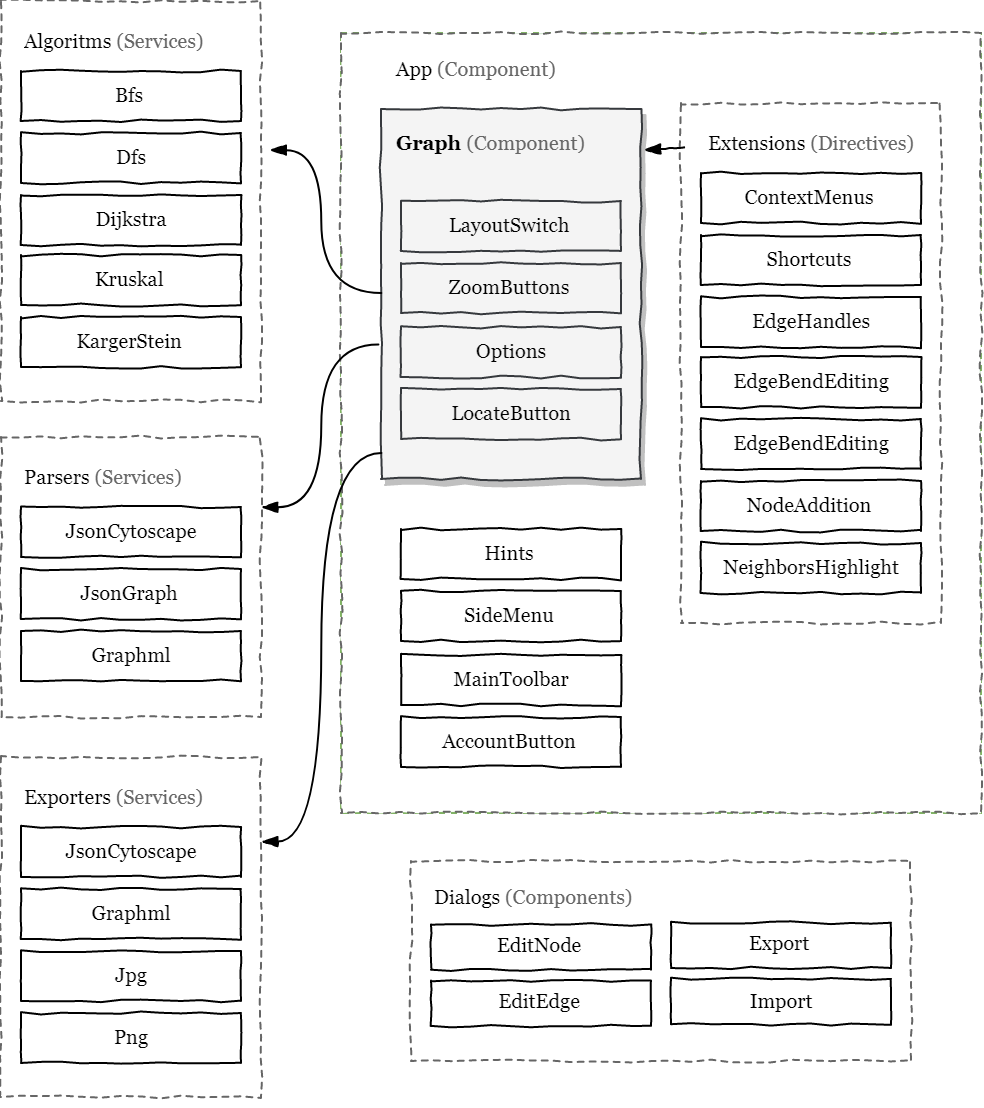
\includegraphics[width=1.1\textwidth]{architecture}}
\captionsetup{justification=centering,aboveskip=24pt}
\caption{Zarys architektury projektu \\ (niektóre komponenty zostały pominięte)}
\label{fig:protractor}\label{fig:architecture}
\end{figure}

\begin{figure}[H]
\centerline{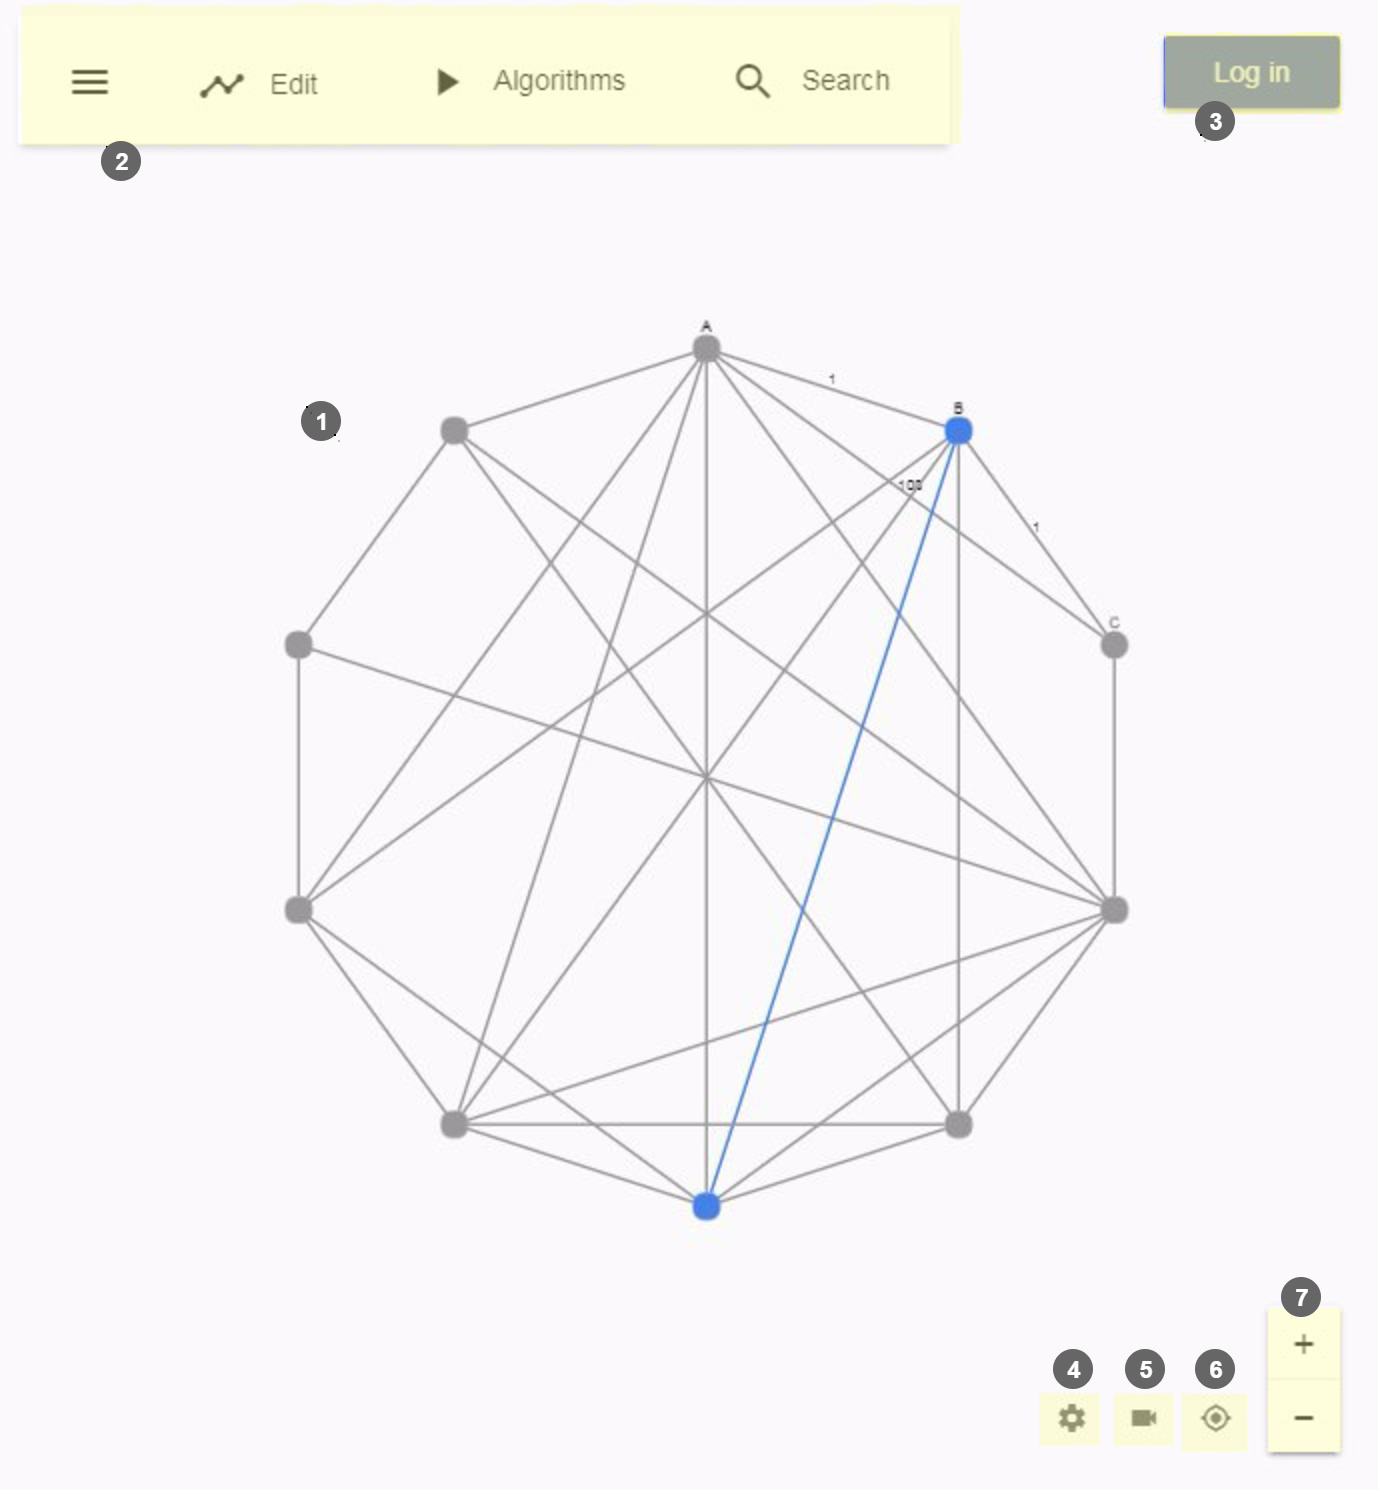
\includegraphics[width=1.0\textwidth]{graphy}}
\captionsetup{singlelinecheck=off}
\caption[Graphy]{
Aplikacja Graphy z zaznaczonymi głównymi komponentami:
\begin{enumerate}
\setlength{\itemsep}{0pt}
\setlength{\parskip}{2pt}
\item \texttt{GraphComponent}
\item \texttt{MainToolbarComponent}
\item \texttt{AccountButtonComponent}
\item \texttt{OptionsButtonComponent}
\item \texttt{LyoutSwitchComponent}
\item \texttt{LocateButtonComponent}
\item \texttt{ZoomButtonsComponent}
\end{enumerate}
}
\label{fig:protractor}
\end{figure}

\section{Zaimplementowane funkcjonalności}

W aplikacji udało się zaimplementować większość funkcjonalności, które zostały opisane w rozdziale \ref{ch:project} pt. ,,Projekt aplikacji''. Są to przede wszystkim:

\begin{itemize}
\setlength\itemsep{0em}
\item tworzenie grafów skierowanych oraz nieskierowanych,
\item importowanie grafu z formatów: GraphML, JSON Graph Format lub z~formatu JSON, z którego korzysta biblioteka Cytoscape.js,
\item eksportowanie do formatu GraphML, formatu JSON obsługiwanego przez Cytoscape.js oraz plików graficznych w formatach JPG i PNG,
\item obsługa podstawowych algorytmów wraz z animacją (BFS, DFS, algorytm Dijkstry, algorytm Kruskala, algorytm Kargera-Steina),
\item tryb edycji: dodawanie wierzchołków poprzez kliknięcie na obszar roboczy (lub z menu kontekstowego); dodawanie krawędzi poprzez przeciąganie (lub z menu kontekstowego),
\item grupowanie wierzchołków,
\item zmiana stylu wierzchołków oraz krawędzi (kolor, kształt, grubość krawędzi, styl linii, wielkość wierzchołków),
\item wyginanie krawędzi,
\item przystosowane menu kontekstowe,
\item obsługa skrótów klawiszowych,
\item wyświetlanie ostatniej akcji wraz z możliwością jej cofnięcia,
\item kopiowanie, wycinanie, wklejanie wierzchołków i krawędzi,
\item wsparcie dla urządzeń mobilnych i z ekranem dotykowym.
\end{itemize}

\section{Niezaimplementowane funkcjonalności i wizja dalszego rozwoju}

Jednakże ze względu na ograniczony czas i szeroki zakres pracy, nie wszystkie funkcjonalności udało się zaimplementować. Należą do nich głównie:

\begin{itemize}
\setlength\itemsep{0em}
\item logowanie użytkownika,
\item wczytywanie i zapisywanie grafów do bazy, na Dropboxie lub na Google Drive,
\item obsługa formatu GEXF,
\item generowanie grafów,
\item wyszukiwanie elementów w grafie,
\item ograniczona liczba algorytmów,
\item udostępnianie grafu,
\item wydajność i obsługa dużych grafów.
\end{itemize}

Logowanie użytkowników i zapis grafów do bazy będzie możliwe po zaimplementowaniu części serwerowej. Dzięki architekturze aplikacji, dodanie gotowego parsera nie powinno być wielkim wyzwaniem. To samo dotyczy dodawania nowych algorytmów. Warto wspomnieć, że jeszcze nie wszystkie algorytmy domyślnie zaimplementowane w bibliotece Cytoscape.js są obecnie wykorzystywane w aplikacji.

Jeśli chodzi o wydajność i obsługę dużych grafów, to nie zostało to sprawdzone. Niewykluczone, że przy dużych grafach aplikacja będzie działać powoli. Wówczas pomocne może okazać się zastosowanie wskazówek zawartych na stronie Cytoscape.js w sekcji dotyczącej wydajności (\cite{cytoscape} \textit{Performance}). Warto będzie również dopisać testy wydajności by móc ją na bieżąco kontrolować. 

Udostępnianie grafów innym użytkownikom w czasie rzeczywistym jest interesującym tematem. Aby to osiągnąć konieczne będzie również dopisanie części serwerowej. Przy obecnym stanie rzeczy, prawdopodobnie najlepszym rozwiązaniem będzie zastosowanie technologii WebSocket, która zapewnia dwukierunkową komunikację pomiędzy serwerem a przeglądarką internetową poprzez protokół TCP. 

Kolejnym interesującym i szerokim zagadnieniem jest integracja z grafowymi bazami danych, np. z bazą Neo4j poprzez protokół Bolt i język zapytań Cypher.

\section{Informacje dla programistów}

\subsection*{Dodawanie nowego parsera}

Aby dodać nowy parser należy:

\begin{enumerate}
\setlength\itemsep{0em}
\item Utworzyć nową klasę \texttt{NowyFormatParser} w pliku o nazwie \\ \texttt{nowy-format-parser.ts} w katalogu \texttt{app/graph/parsers/}.

\item Podziedziczyć po klasie \texttt{Parser} i zaimplementować dwie metody: \\ \texttt{parse()} oraz \texttt{id()}.

\item Zarejestrować nowego \textit{providera} w \texttt{GraphComponent} poprzez dodanie do tablicy \texttt{providers} nowego obiektu:\\
\texttt{\{provide: Parser, useClass: NowyFormatParser, multi: true\},}

\item Dodać nowy format w serwisie \texttt{GraphFormatsService} poprzez dodanie do tablicy zwracanej przez metodę \texttt{getSupportedFormats()} nowego obiektu : \\
\texttt{\{id: '', name: '', extensions: ['']}\}, \\ 
gdzie: \\
\texttt{id} -- wartość zwracana przez metodę \texttt{id()} w klasie \texttt{NowyFormatParser}, \texttt{name} -- nazwa wyświetlana na liście w oknie do importowania grafu,\\ \texttt{extensions} -- tablica dopuszczalnych rozszerzeń dla danego formatu.
\end{enumerate}

\subsection*{Dodawanie nowego eksportera}

\subsection*{Dodawanie nowego algorytmu}

\subsection*{Dodawanie nowego skrótu klawiszowego}

\section{Testy}\label{sec:tests}

\subsection*{Testy jednostkowe}

Projekt wygenerowany przez Angular CLI domyślnie dostarcza skonfigurowane środowisko do testów jednostkowych (Karma, Jasmine). Testy możemy uruchomić komendą \texttt{ng test}. Przy dodawaniu nowego komponentu czy serwisu od razu tworzony jest plik z testami do niego. W aplikacji zostało napisanych kilka przykładowych testów jednostkowych (podczas dalszego rozwoju aplikacji konieczne będzie dokończenie tych testów).

Projekt został również zintegrowany z Travis CI. Jest to środowisko ciągłej integracji (ang. \textit{continuous integration}). Przy każdym wypchnięciu zmian do głównej, zdalnej gałęzi na GitHubie (\texttt{git push origin master}) projekt jest budowany na zdalnym serwerze i uruchamiane są wszystkie testy jednostkowe. Zapewnia to kontrolę nad tym, aby projekt stale budował się poprawnie. Gdy podczas budowania projektu wystąpi jakiś błąd, to wysyłany jest mail z informacją o niepowodzeniu.

\subsection*{Testy \textit{end-to-end}}

Angular CLI dostarcza również skonfigurowane środowisko do testów \textit{end-to-end}, które jest oparte na platformie programistycznej Protractor. Testy te możemy uruchomić poleceniem \texttt{ng e2e}. 

Protractor jest aplikacją Node.js wykorzystującą WebDriverJS. Uruchamia on całą aplikację w przeglądarce (w trybie graficznym lub \textit{headless} -- bez garficznego interfejsu użytkownika) i komunikuje się z nią poprzez Chrome Drivera (lub Selenium Drivera) co zostało przedstawione na rysunku \ref{fig:protractor}. W~praktyce oznacza to, że testy operują na aplikacji tak, jak gdyby robił to prawdziwy użytkownik (np. kliknięcie myszką w dany element, przesunięcie kursora myszki w wyznaczone miejsce, naciśnięcie danych znaków na klawiaturze). 

\begin{figure}[H]
\centering
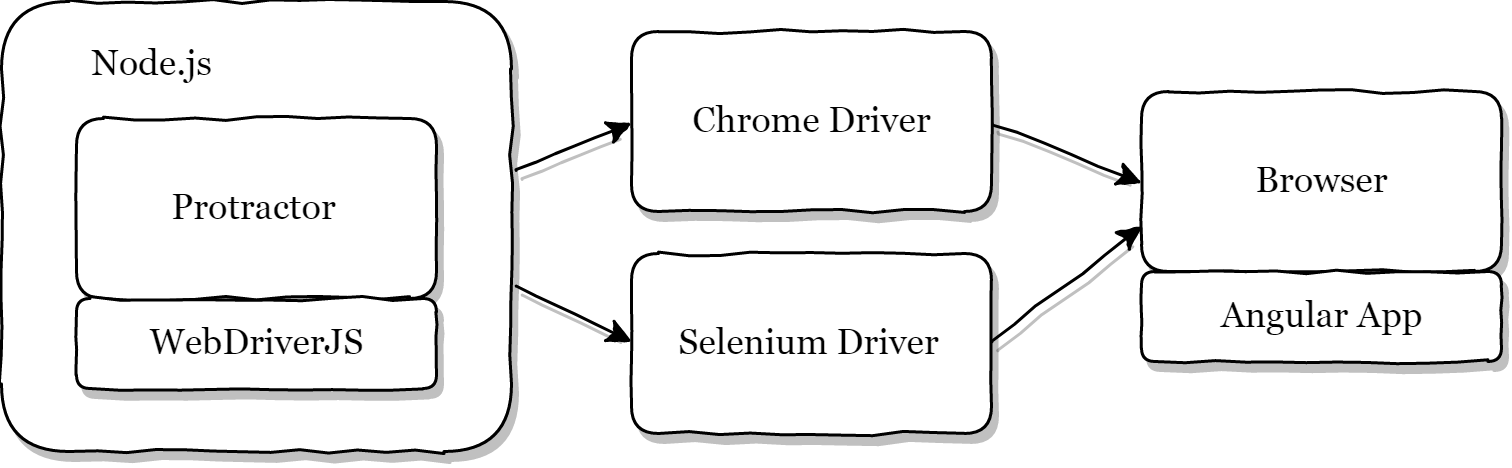
\includegraphics[width=\textwidth]{protractor}
\caption{Protractor -- zasada działania}
\label{fig:protractor}
\end{figure}

Platforma ta pozwoliła stworzyć testy automatyczne, które sprawdzają m.in. czy menu kontekstowe zawiera odpowiednie elementy zarówno w trybie widoku jak i edycji, czy poprawnie działają skróty klawiszowe, czy kliknięcie na graf w trybie edycji (i tylko w trybie edycji) utworzy nowy wierzchołek, czy graf poprawnie się eksportuje. 

Jako że Cytoscape.js korzysta z HTML5 Canvas do wyświetlania elementów grafu, sprawdzenie czy np. został dodany lub usunięty jakiś wierzchołek było nie lada wyzwaniem, ponieważ testowanie czy dane piksele mają odpowiedni kolor jest nieco kłopotliwe. W chwili obecnej udało się to osiągnąć poprzez weryfikację wyeksportowanego grafu (dzięki czemu od razu sprawdzana jest funkcjonalność eksportu). W przyszłości, gdy liczba testów wzrośnie, można rozważyć dodanie do aplikacji okna dialogowego wyświetlającego informacje o grafie -- powinno to przyspieszyć czas wykonywania się testów.

Podobnie jak testy jednostkowe, testy \textit{end-to-end} wykonują się zdalnie na serwerze Travis CI po każdorazowym wypchnięciu zmian do głównej gałęzi. Aby testy poprawnie działały na zdalnej maszynie, potrzebne było określenie konkretnego wymiaru okna przeglądarki oraz dokładnych punktów, w które ma klikać test. Było to konieczne z tego względu, ponieważ zdarzyło się, że test, który przy lokalnym uruchomieniu klikał na pustą przestrzeń, dodając przy tym nowy wierzchołek, przy uruchomieniu zdalnym trafiał w wierzchołek, zaznaczając go. 

Temat testowania \textit{end-to-end} takiej aplikacji jest ciekawy i w dalszym jej rozwoju warto, aby powstawały kolejne scenariusze testowe. Dzięki tym testom zyskujemy gwarancję, że aplikacja działa poprawnie jako całość oraz że wszystkie komponenty współpracują ze sobą tak, jak powinny. Takiej gwarancji nie mogą dać same testy jednostkowe. 

\subsection*{Testy manualne}

Aplikacja została przetestowana manualnie na laptopie pod przeglądarkami Chrome 59, Firefox 54 oraz Internet Explorer w wersji 11. Aby aplikacja poprawnie uruchomiła się pod przeglądarką Internet Explorer, konieczne było dodanie \textit{polyfilli}\footnote{Termin ten oznacza kawałek kodu, który implementuje nową funkcjonalność, która w starszych przeglądarkach internetowych nie jest dostępna.}, które w projekcie wygenerowanym przez Angular CLI nie są domyślnie importowane \cite{duveau}. Według W3Schools w chwili obecnej użycie przeglądarki IE wynosi około 4,6\% \cite{w3schools}. Gdy liczba ta będzie bliska zeru oraz gdy nowe przeglądarki będą w pełni implementować funkcjonalności uzupełniane przez ów \textit{polyfille}, wówczas będzie można je z powrotem wyłączyć (zakomentować odpowiednie linijki w pliku \texttt{polyfills.ts}). Dzięki temu wynikowy kod JavaScript zostanie pomniejszony o około 62 KB \cite{angular-browser-support}. 

Aplikacja została również sprawdzona na tablecie Lark Ultimate X4 10.1 3G IPS z systemem operacyjnym Android 6.0.0 i przeglądarką Chrome w wersji 55, który posiada 10,1 calowy ekran. Korzystanie z aplikacji na urządzeniu tego typu jest możliwe. Użytkownik jest w stanie wyświetlić graf, zmieniać ustawienie wierzchołków, dodawać nowe wierzchołki oraz krawędzie, uruchamiać algorytmy oraz wyeksportować graf. Po wstępnych testach wynika, że poprawnie działają wszystkie gesty, takie jak: przeciąganie, stuknięcie, powiększanie i oddalanie dwoma palcami czy otwieranie menu kontekstowego poprzez stuknięcie dwoma palcami. 

Jedynym mankamentem jest zaznaczanie przez pole (ang. \textit{box selection}), które na urządzeniach dotykowych możemy osiągnąć poprzez przesuwanie trzema palcami. Niestety mechanizm ten pozostawia wiele do życzenia. Na komputerze stacjonarnym czy laptopie, gdy mamy dostępną standardową klawiaturę, możemy użyć klawiszy modyfikujących (\texttt{Control}, \texttt{Shift}, \texttt{Alt}, \texttt{Command}), aby zaznaczać kilka wierzchołków oraz krawędzi. Na urządzeniu dotykowym w chwili obecnej jest to praktycznie niemożliwe i jeśli aplikacja ma być w przyszłości rozwijana, to konieczne będzie rozważenie dodania dodatkowej opcji w menu kontekstowym służącej do zmiany zaznaczenia lub przycisku przełączającego pomiędzy trybami przesuwania widoku i zaznaczania. 

Ponadto aplikacja Graphy została sprawdzona na telefonie o przekątnej ekranu 4,7 cala i rozdzielczości 540$\times$960 px. Korzystanie z niej było również możliwe i wygląda na to, że wszystkie funkcjonalności działają poprawnie. Dzięki zastosowaniu reguły \texttt{@media} z CSS3 możliwe było dostosowanie interfejsu pod tak niską rozdzielczość (główne menu jest ukrywane i wyświetlane w bocznym, rozsuwanym menu). 

